%ici je veux présenter la méthodologie et les données que j'ai utilisées 

\section{Data and Methods}

The general workflow for integrating time-series data in a PH model is depicted in \pref{fig:workflow}, in the following sections we 
detail some of the workflow steps.
% and comprises the following steps:
\begin{figure}[H]
 \centering
 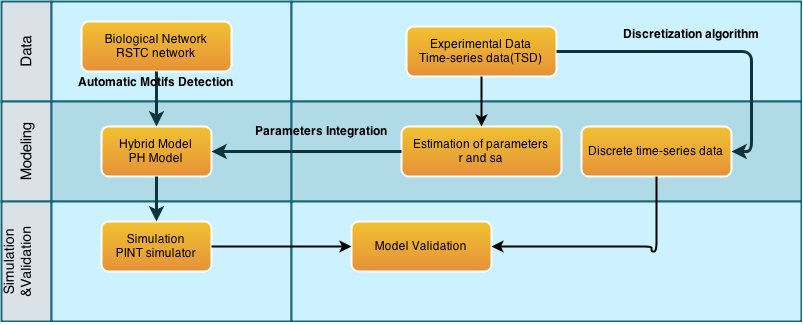
\includegraphics[width=4.1in,height=2in]{images/workflow-2.png}
\caption{{\bf Integrating stochastic and temporal information in a large-scale discrete biological model. These parameters are rate (r) and the stochasticity absortion factor (sa) which 
will be presented later in \ref{sssec:EPTSD}.}} 
 \label{fig:workflow}
\end{figure}


\subsection{Data}

\subsubsection{Interaction graph.}
% \paragraph{The RSTC Network}
\label{ssec:RSTC}
The interactions of the biological system under study were represented in
 an RSTC network, which stands for  multi-layer receptor-signaling-transcription-cell state network and that was generated from the Pathway Interaction Database (PID).
In order to build this network one needs to select a set of seed nodes related to the biological process studied.
For our case study, the seed nodes were:  (1) \emph{E-cadherin}, which is a protein having Calcium binding domains and which plays an important role in cell adhesion;
(2) the $12$ significantly differentially expressed genes accross the $10$ time-points; and (3) the cell states of keratinocytes-differentiation and cell-cycle-arrest. 
The network was extracted automatically from the whole content of the NCI-PID database by using a subgraph algorithm to link the seed nodes \cite{guziolowski2012automatic}. 
In \pref{fig:network} we show the RSTC network obtained. 


\begin{definition}[RSTC Network] \label{def:RSTCDef}
A \emph{RSTC Network} $N$ is a couple $(V,E)$, where:
\begin{itemize}
\item $V =V_{T} \bigcup V_{I} $ is the finite set of \emph{nodes};
 with 
  $V_{T} = \{v_{1t},v_{2t}, \dots ,v_{n1t} \} $ the set of terminal nodes;
  $V_{I} = \{v_{1i},v_{2i}, \dots ,v_{n2i} \} $ the set of transient nodes.
\item $E = \{e_{1},e_{2}, \dots, e_{m} \}$ is the set of edges. $ E \subseteq (V_{T} \times V_{T}) \bigcup (V_{T} \times V_{I}) 
\bigcup (V_{I} \times V_{T})$
\end{itemize}
\end{definition}

In this definition, terminal nodes can be \modCG{mRNA expression}, proteins, complexes, cellular states, biological processes and positive conditions. 
On the other side, transient nodes can be transcriptions, translocations, modifications and compounds. Edges are of different types:
activation (agent), inhibition, output, input and protein-family-member.

%\modCG{

\begin{definition}[Pattern] \label{def:pattern}

A pattern can be defined as an atomic set of biological components and thier interacting roles. 

\end{definition}

\modCG{
First colonne of table \ref{table_patterns} shows us some examples of patterns that we can found in a RSTC Network.
}
%}

\begin{figure}[!p]
 \centering
 \includegraphics[width=12cm, height=10cm]{images/net_cg_v3.png}
\caption{{\bf  Interaction graph linking E-cadherin with 12 genes of the time-series dataset.} Blue nodes correspond to E-cadherin entities, red or green, to time-series genes, 
and cyan nodes to cellular processes. The graph is composed of $293$ nodes and $375$ edges (interactions).
The set of nodes are composed of terminal nodes (proteins, complexes, \modCG{ mRNA expression}, cellular state, biological processes and positive conditions) and of transient
nodes (transcriptions, translocations, modifications and compounds). The set of edges are composed of interactions of type activation, inhibition, output, 
input and protein-family-member.} 
 \label{fig:network}
\end{figure}

%description des données
\subsubsection{Time-series microarray dataset.}
\label{SECTSD}
\modCG{We use the time-series microarray data from Calcium stimulated human keratinocyte cells 
 measured at $10$ time-points (1h, 2h, 3h, 4h, 5h, 6h, 8h, 12h, 18h, 24h). 
The expression levels were measured in $log_2$; the expression of a gene at an 
specific time point is compared with respect to a control condition (gene expression in a kerationocyte cell without Calcium stimulation).
We selected genes, which mRNA expression $e$ was significantly ($log_2(e) \ge 1$) up-regulated  or 
significantly ($log_2(e) \le -1.0$) down-regulated in at least one time point compared to control.
From this procedure $200$ \modCG{mRNA expression} transcripts were selected. 
We included in our model a subset of $12$ of the $200$ selected (see \pref{fig:tsd})
because these 12 genes had upstream regulatory mechanisms when querying the 
PID-NCI database and therefore were connected in the interaction graph to the E-cadherin node}.
%The full dataset (data not shown) was produced by the German Cancer Research Center (DKFZ) and is currently in the process
%of being published.  

\begin{figure}[H]
\centering
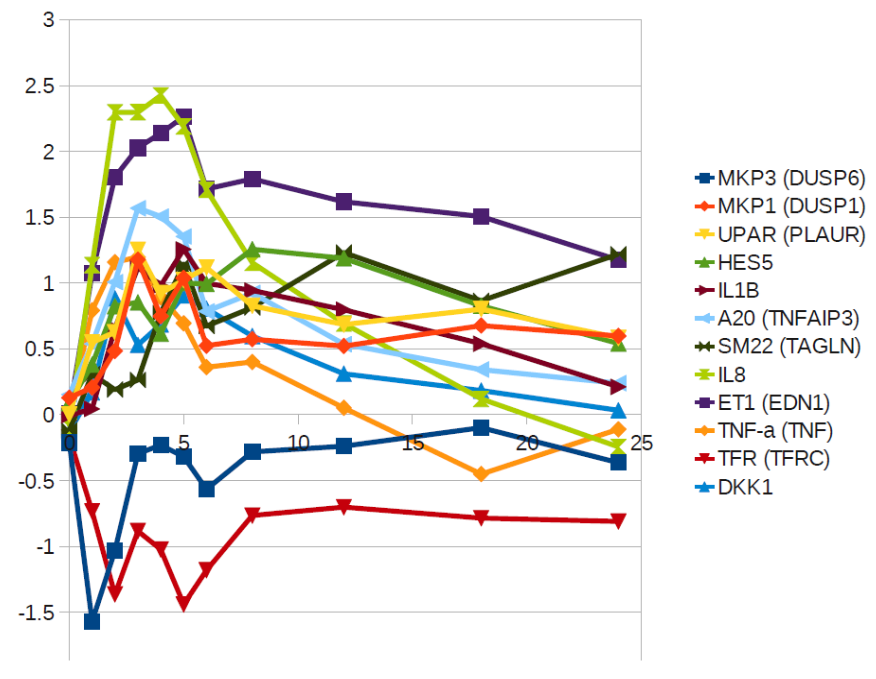
\includegraphics[width=3.5in, height=2.5in]{images/12genes.png}
\caption{\bf Relative expression of selected mRNA upon Calcium stimulation.} The $X$ axis represents time duration of the experiment measured in hours. 
The $Y$ axis represents the $log_{2}$ expression level of genes with respect to control.
\label{fig:tsd}
\end{figure}


\subsection{The Process  Hitting Framework}
\label{ssec:PH}

%We present here the Process Hitting framework \cite{PMR10-TCSB} which will enable us to model 
%biological network.

%\vspace{3mm}

Process Hitting (PH) gathers a finite number of concurrent processes grouped into a finite set of sorts.
A sort stands for a component of a biological system while a process, which belongs to a unique sort, stands
for one of its expression levels. At any time exactly one process of each sort is present. A state of the 
PH corresponds to such a set of processes. We denote here a process by $a_i$ where $a$ 
is the sort and $i$ is the process identifier within the sort $a$.
The concurrent interactions between processes are defined by a set of \emph{actions}.
Actions describe the replacement of a process by another of the same sort conditioned by the presence 
of at most one other process in the current state. An action is denoted by $\PHfrappe{a_i}{b_j}{b_k}$, 
which is read as ``$a_i$ \emph{hits} $b_j$ to make it bounce to $b_k$'', where $a_i,b_j,b_k$ are 
processes of sorts $a$ and $b$, called respectively \emph{hitter}, \emph{target} and \emph{bounce} of 
the action.

\begin{definition}[Process Hitting] \label{def:PH}
A \emph{Process Hitting} is a triple $(\PHs,\PHl,\PHa)$, where:
\begin{itemize}
\item $\PHs = \{a,b,\dots\}$ is the finite set of \emph{sorts};
\item $\PHl = \prod_{a\in\PHs} \PHl_a$ is the set of states with $\PHl_a = \{a_0,\dots,a_{l_a}\}$
the finite set of \emph{processes} of sort $a\in\Sigma$ and $l_a$ a positive integer, with $a\neq b\Rightarrow \PHl_a \cap \PHl_b = \emptyset$;
\item $\PHa = \{ \PHfrappe{a_i}{b_j}{b_k} \in \PHl_a \times \PHl_b \times \PHl_b \mid (a,b) \in \PHs^2
  \wedge b_j\neq b_k \wedge a=b\Rightarrow a_i=b_j\}$ is the finite set of \emph{actions}.
\end{itemize}
\end{definition}

\noindent
Given a state $s\in \PHl$, the process of sort $a\in\PHs$ present in $s$ is denoted by $\PHget{s}{a}$.
An action $h=\PHfrappe{a_i}{b_j}{b_k} \in \PHa$ is \emph{playable} in $s \in L$ if and only if $\PHget{s}{a}=a_i$ and $\PHget{s}{b} = b_j$.
In such a case, $(s\play h)$ stands for the state resulting from playing the action $h$ in $s$, with
$\PHget{(s\play h)}{b} = b_k$ and $\forall c \in \PHs, c \neq b, \PHget{(s\play h)}{c} = \PHget{s}{c}$.
In order to model the fact that a molecule in the interaction graph is influenced by various molecules, two 
types of modeling-scenarios can be proposed: cooperation and synchronization.

\subsubsection{Modeling cooperation}

The cooperation between processes to make another process bounce can be
expressed in PH by building a \emph{cooperative sort}~\cite{PMR10-TCSB}.
\pref{fig:runningPH} shows an example of a cooperative sort $ab$ between sorts $a$ and $b$,
which is composed of 4 processes (one for each sub-state of the presence of processes in $a$ and $b$).
For the sake of clarity, processes of $ab$ are indexed using the sub-state they represent.
Hence, $ab_{01}$ represents the sub-state $\PHstate{a_0,b_1}$, and so on.
Each process of sort $a$ and $b$ hits $ab$, which makes it bounce to the process reflecting the status of the sorts $a$
and $b$ (e.g., $\PHfrappe{a_1}{ab_{00}}{ab_{10}}$ and $\PHfrappe{a_1}{ab_{01}}{ab_{11}}$).
Then, to represent the cooperation between processes $a_1$ and $b_1$,
the process $ab_{11}$ hits $c_1$ to make it bounce to $c_2$ instead of
independent hits from $a_1$ and $b_1$.
The same cooperative sort is used to make $a_0$ and $b_0$ cooperate to hit $c_1$ and make it bounce to $c_0$.
Cooperation sort allows to model the fact that two components cooperate to hit another component.
\subsubsection{Modeling synchronization}
\label{sssec:synchronization}

The synchronization sort implements another type of cooperation. If we refer to the example of
\pref{fig:runningPH} left, we can similarly construct a \emph{synchronization sort} $ab$ between sorts $a$ and $b$, defined with also 
4 processes. Then, component $c$ is activated ($c_1$ bounces to $c_2$ or $c_0$ bounces to $c_1$) if either  $a$ or $b$ are activated. Therefore, each one of 
these processes $ab_{01}$, $ab_{10}$, $ab_{11}$ can activate $c$.  In order to inhibit $c$, both sorts, $a$ and $b$, need to be 
in the sub-state $0$, i.e. $ab_{00}$. Notice that this rule is a combination of OR logical gates for activation and AND logical gates for inhibition.
Imposing the synchronization sort to model a target component regulated independently by multiple predecessors avoids oscillations in the behavior of the target component over time. 
These oscillations appear because each predecessor can independently activate the target component when it is active,
but when one predecessor is inhibited, it will inhibit the target component. This competition between the predecessors
generates oscillations on the target component.  


\begin{example}
\pref{fig:runningPH} represents a PH $(\PHs,\PHl,\PHa)$ with $\PHs = \{a,b,c,ab\}$, and:
\begin{align*}
\PHl_a &= \{a_0,a_1\},\\
\PHl_b &= \{b_0, b_1\},\\
\PHl_{ab} &= \{ab_{00}, ab_{01}, ab_{10}, ab_{11}\},&\\
\PHl_c &= \{c_0, c_1, c_2\}.
\end{align*}
This example models a Biological Regulatory Network (BRN) where the component $c$ has three qualitative levels, components $a$ and $b$ are Boolean and $ab$ is a cooperative sort.
In this BRN, $ab$ inhibits $c$ at level $2$ through the cooperative sort $ab$ (e.g. $\PHfrappe{ab_{00}}{c_2}{c_1}$, $\PHfrappe{ab_{00}}{c_1}{c_0}$) while $a$ and $b$ activate $c$  
through the cooperative sort $ab$ (e.g. $\PHfrappe{ab_{11}}{c_0}{c_1}$ $\PHfrappe{ab_{11}}{c_1}{c_2}$ ). Indeed, the reachability of $c_2$ and $c_0$ 
is conditioned by a cooperation of $a$ and $b$ as explained above.

\begin{figure}[H]
%\centering
\begin{minipage}{0.1\linewidth}
\centering
\scalebox{0.9}{
\begin{tikzpicture}[grn]
\path[use as bounding box] (-0.2,-0.7) rectangle (3.5,0.7);
\node[inner sep=0] (a) at (1,2) {a};
\node[inner sep=0] (b) at (1,0) {b};
\node[inner sep=0] (c) at (3,1) {c};
\path[->]
  (b) edge node[elabel, above=-3pt] {$+$} (c)
  %(c) edge node[elabel, above=-5pt] {$1+$} (a)
  (a) edge node[elabel, above=-3pt] {$+$} (c);
\end{tikzpicture}
}
\end{minipage}
%%%%%%%%%%%%%%%%%%%%%%%%%%%%%%%%%%%%%%%%
\hspace{2cm}
%%%%%%%%%%%%%%%%%%%%%%%%%%%%%%%%%%%%%%%%%
\begin{minipage}{0.7\linewidth}
\centering
\scalebox{0.7}{
\begin{tikzpicture}
\path[use as bounding box] (-2,-5.2) rectangle (7,0.7);

\TSort{(0,0)}{a}{2}{t}
\TSort{(0,-3.8)}{b}{2}{b}
\TSort{(4.5,-3)}{c}{3}{r}

\TSetTick{ab}{0}{00}
\TSetTick{ab}{1}{01}
\TSetTick{ab}{2}{10}
\TSetTick{ab}{3}{11}
\TSort{(-0.5,-2)}{ab}{4}{b}


\THit{a_1}{bend right}{ab_0}{.north}{ab_2}
\THit{a_1}{bend right}{ab_1}{.north}{ab_3}
\THit{a_0}{}{ab_2}{.north west}{ab_0}
\THit{a_0}{}{ab_3}{.north west}{ab_1}

\THit{b_0}{}{ab_1}{.south}{ab_0}
\THit{b_0}{}{ab_3}{.south}{ab_2}
\THit{b_1}{}{ab_0}{.south}{ab_1}
\THit{b_1}{}{ab_2}{.south}{ab_3}

\path[bounce, bend right=25]
\TBounce{ab_2}{}{ab_0}{.north east}
\TBounce{ab_3}{}{ab_1}{.north east}
;
\path[bounce, bend left=80, distance=30]
\TBounce{ab_0}{}{ab_2}{.north}
\TBounce{ab_1}{}{ab_3}{.north}
;
\path[bounce, bend right]
\TBounce{ab_0}{}{ab_1}{.west}
\TBounce{ab_2}{}{ab_3}{.west}
;
\path[bounce, bend left]
\TBounce{ab_3}{}{ab_2}{.east}
\TBounce{ab_1}{}{ab_0}{.east}
;

\THit{ab_3}{thick}{c_1}{.north west}{c_2}
\THit{ab_0}{thick,bend right=130, in=305, distance=140}{c_1}{.south east}{c_0}
\path[bounce, bend left=40]
\TBounce{c_1}{thick}{c_2}{.south west}
\TBounce{c_1}{thick}{c_0}{.north east}
;

\THit{ab_3}{thick}{c_0}{.north west}{c_1}
\THit{ab_0}{thick,bend right=130, in=305, distance=140}{c_2}{.south east}{c_1}
\path[bounce, bend left=40]
\TBounce{c_0}{thick}{c_1}{.south west}
\TBounce{c_2}{thick}{c_1}{.north east}
;
\end{tikzpicture}
}
\end{minipage}

\caption{ \label{fig:modelingBRN}
{\bf (Left)~biological pattern example.}
Nodes represent molecules (components) and edges, interactions.
In this pattern components $a$ and $b$ cooperate to activate $c$.
{\bf (Right)~equivalent PH model} \label{fig:runningPH}
with four sorts: three components ($a$, $b$ and $c$) and a cooperative sort ($ab$).
Actions targeting processes of $c$ are drawn as thick lines.
}
\end{figure}

\end{example}




%la traduction automatique des patterns d'un réseau
\subsection{Model construction (from RSTC to PH)}

\subsubsection{Modeling the RSTC network as a PH model.}


%\paragraph{Modeling biological patterns to PH model}

%Here is the first and the most important part of this work. 
In order to model the RSTC network as a PH model we select known biological regulatory patterns (atomic set of biological components and their interacting roles), represented 
as biochemical reactions in the RSTC network and propose their PH representation. Table \ref{table_patterns} shows some examples of this transformation. 

%les ajouts pour les patterns 
The automatic pattern selection and PH model generation algorithms use two procedures. 
%
The first takes as parameter argument the graph and automatically browses it node by node and detects all patterns in the graph. 
For each node (output node of the pattern) we  call a recursive procedure,
that  allows  to detect a minimal set of nodes (input node of the pattern) that has a direct influence over that node. 
This set of nodes plus the output node and the way  input and output are linked form a pattern. 
The type of a pattern is determined by the type of the output node, the type of regulations that arrive to that node and the type of input nodes of the pattern. 
Consequently, the algorithm of patterns detection returns the pattern 
and its type to another procedure  which  translates the pattern into the PH formalism. This transformation  takes care of different cases (cooperation, synchronization, simple activation, simple inhibition, etc.)


% les détails sur comment les patterns sont choisis 
For example a molecule $a$ cooperating with a molecule $b$ to activate a molecule $c$ (\pref{fig:runningPH}, left), is a regulatory pattern because it is a protein-complex biochemical reaction that appears recurrent times.  
We model this pattern by four sorts (\pref{fig:runningPH}, right) $a$, $b$, $c$ and $ab$. Sorts $a$, $b$ and $c$
stand for components $a$, $b$ and $c$. The cooperative sort $ab$ is introduced in order to characterize constraints on the components $a$ and $b$.
In the RSTC network, we find  $25$ regulatory patterns. We show some examples in Table \ref{table_patterns}.     %TODO

\begin{table}[!t]
\renewcommand{\arraystretch}{1.3}
\caption{Examples of patterns}
\label{table_patterns}
\centering
\begin{tabular}{|c|c|M{4cm}|}
\hline
\bfseries Biological Patterns

&

\bfseries PH Transformations

&

\bfseries Descriptions \tabularnewline 
\hline
\begin{tikzpicture}
\node[scale=0.65] (sa1) at (0,0){\begin{tikzpicture}[auto]
\path[use as bounding box] (-0.7,-0.3) rectangle (2.5,2);

\node[qgre] (a) at (0,1) {a};
\node[mod] (i) at (1,1) {i};
\node[qgre] (b) at (2,1) {b};
\node[es] (d) at (1,1.5) {Simple activation};

\path
 (a) edge[act] (i)
 (i) edge[st]  (b);
\end{tikzpicture}};
\end{tikzpicture}

&


\begin{tikzpicture}
%\exphpatact
\node[scale=0.5] (sa) at (0,0) {\begin{tikzpicture}
\path[use as bounding box] (-0.5,-0.5) rectangle (2.5,2.5);

\TSort{(0,0.5)}{a}{2}{l}
\TSort{(2,0.5)}{b}{2}{l}
%\TSort{(6,1)}{z}{3}{r}

\THit{a_1}{}{b_0}{.west}{b_1}
\THit{a_0}{}{b_1}{.west}{b_0}
%\THit{a_0}{out=250,in=200,selfhit}{a_0}{.west}{a_1}

\path[bounce,bend left]
\TBounce{b_0}{}{b_1}{.south}
\TBounce{b_1}{bend right}{b_0}{.north}
%\TBounce{a_0}{}{a_1}{.south}
;
\end{tikzpicture}};
\end{tikzpicture}

&

This pattern model the activation of the component b by the component a.\tabularnewline
\hline

\begin{tikzpicture}
\node[scale=0.65] (si1) at (0,0){\begin{tikzpicture}[auto]
\path[use as bounding box] (-0.7,-0.3) rectangle (2.5,2);

\node[qgre] (a) at (0,1) {a};
\node[mod] (i) at (1,1) {i};
\node[qgre] (b) at (2,1) {b};
\node[es] (d) at (1,1.5) {Simple inhibition};
\path
 (a) edge[inh] (i)
 (i) edge[st]  (b);
 \end{tikzpicture}};
\end{tikzpicture}

&

\begin{tikzpicture}
%\exphpatact
\node[scale=0.5] (sa) at (0,0) {\begin{tikzpicture}
\path[use as bounding box] (-0.5,-0.5) rectangle (2.5,2.5);

\TSort{(0,0.5)}{a}{2}{l}
\TSort{(2,0.5)}{b}{2}{l}
%\TSort{(6,1)}{z}{3}{r}

\THit{a_1}{}{b_1}{.west}{b_0}
\THit{a_0}{}{b_0}{.west}{b_1}
%\THit{a_0}{out=250,in=200,selfhit}{a_0}{.west}{a_1}

\path[bounce,bend left]
\TBounce{b_1}{bend right}{b_0}{.north}
\TBounce{b_0}{}{b_1}{.south}
%\TBounce{a_0}{}{a_1}{.south}
;
\end{tikzpicture}};
\end{tikzpicture}

&

This pattern model the inhibition of the component b by the component a\tabularnewline
\hline

\begin{tikzpicture}
\node[scale=0.65] (sai1) at (0,0){\begin{tikzpicture}[auto]
\path[use as bounding box] (-0.7,-0.3) rectangle (2.5,3);
\node[qgre] (a) at (0,2) {a};
\node[mod] (i) at (1,1) {i};
\node[qgre] (b) at (0,0) {b};
\node[qgre] (c) at (2,1) {c};
\node[es] (d) at (1,3) {Activation or inhibition};

\path
 (a) edge[act] (i)
 (b) edge[inh] (i)
 (i) edge[st]  (c);
\end{tikzpicture}};
\end{tikzpicture}


&

\begin{tikzpicture}
%\exphpatact
\node[scale=0.5] (sai) at (0,0) {\begin{tikzpicture}
\path[use as bounding box] (-0.5,-0.5) rectangle (2.5,5.5);

\TSort{(0,0)}{a}{2}{l}
\TSort{(0,3)}{b}{2}{l}
\TSort{(2,1)}{c}{2}{r}

\THit{a_1}{}{c_0}{.west}{c_1}
\THit{a_0}{}{c_1}{.west}{c_0}
\THit{b_1}{}{c_1}{.west}{c_0}
\THit{b_0}{}{c_0}{.west}{c_1}

%\THit{a_0}{out=250,in=200,selfhit}{a_0}{.west}{a_1}

\path[bounce,bend left]
\TBounce{c_1}{bend right}{c_0}{.north}
\TBounce{c_0}{}{c_1}{.south}
%\TBounce{a_0}{}{a_1}{.south}
;
\end{tikzpicture}};
\end{tikzpicture} 

&

This pattern model either the activation of the component c by the component a or the inhibition of the 
component c by the component b \tabularnewline
\hline
\end{tabular}
\end{table}


%%%%%%%%%%%%%%%%%%%%%%%%%%%%%%%%%%%%%%%%%%%%%%%%%%%%%%%%%%%%%%%%%%%%%%%%%%

\subsubsection{Estimating the parameters for the PH-simulation from time-series gene expression data.}
\label{sssec:EPTSD}
%peut etre penser à faire un schéma

Since the simulation of the execution of the PH actions is done stochastically, we need to relate each action with temporal 
and stochastic parameters introduced into the PH framework to achieve dynamic refinement \cite{PMR10-TCSB}. 
To fire an action in the PH framework we need to provide two parameters: (1) the rate $r=t^{-1}$, where $t$ is the mean time of firing an action,
and (2) the stochasticity absorption factor $sa$, which is introduced to control the variance of firing an action.


\begin{figure}[H]
\centering

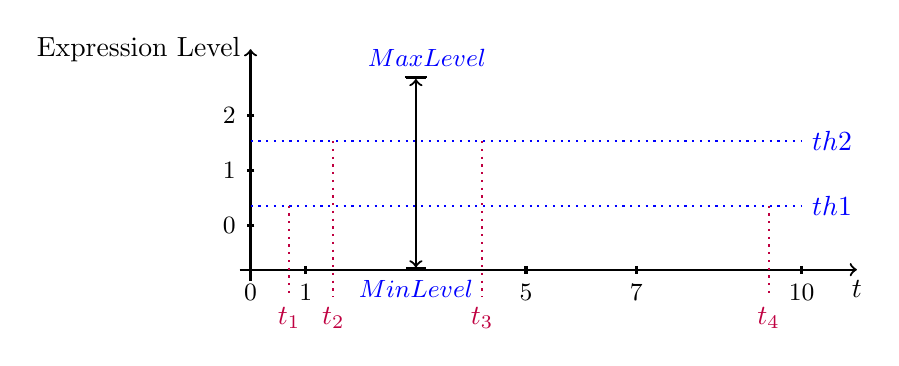
\begin{tikzpicture}[scale = 0.7]
       
    
	      \draw[thick, ->] (-.2,0)--(11,0) node[below]{$t$};
	      \foreach \t in {0,1,5,7,10}
	      \draw[very thick] (\t,2pt)--(\t,-2pt) node[below,black]{\small\t};

	      \draw[thick, ->] (0,-.2)--(0,4) node[left]{Expression Level};
	      \foreach \y in {0,1,2}
               \draw[very thick] (2pt, \y+0.8 )--(-2pt, \y+0.8 ) node[left,black]{\small\y};
           
	      \draw[thick] plot[mark=ball,mark size=1pt] file {illustration.txt};
    
	      %\pause
	      \draw[thick] (2.8,3.5) -- (3.2,3.5) node[above,blue]{\small $MaxLevel$};
	      %\draw[thick,|<->|] (-.2,-.2) -- (.2,-.2) node[below,blue]{};
	      %\pause
	      \draw[thick,|<->|] (3,0)node[below,blue]{\small $MinLevel$} -- (3,3.5);
	      %\pause
	      \draw[thick,dotted,blue] (0,1.16) -- (10,1.16) node[right]{$th1$}; 
	      \draw[thick,dotted,blue] (0,2.33) -- (10,2.33) node[right]{$th2$}; 
	      %\pause
	      \draw[thick,dotted,purple] (0.7,1.16) -- (0.7,-.5) node[below]{$t_{1}$};
	      %\pause
	      \draw[thick,dotted,purple] (1.5,2.33) -- (1.5,-.5) node[below]{$t_{2}$};
	      %\pause
	      \draw[thick,dotted,purple] (4.2,2.33) -- (4.2,-.5) node[below]{$t_{3}$};
	      %\pause
	      \draw[thick,dotted,purple] (9.4,1.16) -- (9.4,-.5) node[below]{$t_{4}$};

           \end{tikzpicture}
	    

\caption{{\bf Estimation of temporal parameters from time series data:} The mean firing time of an action that makes a
component (\modCG{mRNA expression}) change of sub-state is estimated as $r_{i}=\frac{1}{t_{i}-t_{i-1}}$. $MaxLevel$ represents the maximum expression of a \modCG{ mRNA expression}, while 
 $MinLevel$, its minimum expression.
The thresholds $th1$ and $th2$ define the PH discrete sub-states (e.g. 0,1,2) of a component according to its gene expression data.
\label{fig:estimationParameter}}
\end{figure}


For the model components which have a measurement in the time-series data we estimate and integrate $r$ and $sa$ parameters in the PH model. 
The rest of the components will be 
assigned default parameters. In order to estimate $r_{i}$ and $sa_{i}$ for each action $h_{i} \in \PHa$, we need to know the different times $t_{i}$  when the action could be fired as illustrated 
in \pref{fig:estimationParameter}. Each  $t_{i}$ represents the time in which we assume that a component moves from one process to another. Therefore the action that leads this 
change must be played with rate $r_{i}=\frac{1}{t_{i}-t_{i-1}}$. The integer $sa$ represents the window of firing the action at rate $r$ : the larger the $sa$, the small the variance around $r$ is. 
\modCG{ Studies \cite{AMSW2012,Batt15092010,RAT2006} have proposed more elaborate methods for parameters estimation from gene expression data. These methods are well adapted in the case of biochemical reactions where 
the concept of threshold is implicit. In the proposed case we assume an explicit threshold. Thus we can use a basic estimation algorithm for temporal and stochastic parameter estimation.}
%TODO citer les méthodes d'estimation connues et dire pourquoi on en avait pas besoin même si elle sont bonnes 

%discretisation des données
\subsubsection{Discretization of time-series data}

Because the output of a PH simulation are discrete traces of PH components, we discretized continuous experimental data to facilitate 
the comparison with simulation outputs.
When looking at the time-series data (see \pref{fig:tsd}) one can distinguish a high level of
activity in early hours [$0h$-$5h$] and a low level in late hours [$5h$-$10h$]. \modCG{ Trend has been confirmed by using the SMA (Simple moving average) function of R package TTR which allows us
to smooth time-series data. We use the SMA function whith paramter $n=2$ and we have more than $50\%$ of time-series data which presented these two levels of activities.}
%TODO rajouter le test effectuer avec R ici et dire un mot sur ce que ça implique en terme de complexité et la référence 
We implemented a discretization method to capture these
two activation times. For each time-series, we introduced two thresholds \emph{th1} and \emph{th2} (see \pref{fig:estimationParameter}): 
$\emph{th1}=\frac{1}{3}(MaxLevel-MinLevel)$ and $\emph{th2}=\frac{2}{3}(MaxLevel-MinLevel)$. 
In this way, the expression level in the range $[0-th1]$ is at level $0$, the one in the range $[th1-th2]$ is at level $1$, and the one in the last range is at
level $2$. 


\subsection{Simulation}
%we give the initial condition for the simulation

We set the same initial conditions to PH components belonging to the same network layer, chosen from the RSTC structure.
These initial conditions are detailed below and summarized in \pref{fig:initialCondition}.
% where we can clearly see the initial values chosen at each layer for our model.
%To run the simulation we need to set initial conditions for the components of our network. Because the components of the network are grouped into 
%layers, the initial conditions will be the same in the different layers. In the following we will present the initial conditions that we have chosen for the different 
%components.

\begin{itemize}
 \item \textbf{Receptor layer: E-cadherin.} We choose the  pulse signal for the input node E-cadherin to be active for a duration of $5$ units times in average. We made this 
 choice to take into account the average time of the Calcium stimuli effect.
 \item \textbf{Signaling layer: signaling proteins.} The components in this layer are activated and inhibited with the same rate and the same stochasticity absorption factor. 
% Nevertheless, 
The actions between a controller component $A$ and a controlled component $B$ are constrained so that 
$B$ is first activated by $A$ and then inhibited.  That is, 
the time interval in which an inhibition action from $A$ to $B$ fires is greater than 
the time interval in which an activation action from $A$ to $B$ fires.
Additionally, these two time intervals must not overlap.
These constraints can be seen as 
%The choice of inhibition parameters must ensure that the time interval in which the inhibition action 
% is firing is greater than the time interval of firing activation action on the same component. Moreover, it should not be any overlap between the two time intervals. These two conditions
% can be seen as 
reachability constraints from the entry  node (E-cadherin) to the output nodes (mRNA expression). The values of these parameters are selected by considering the delay of signal transduction from the entry
 node to the output nodes.
 \item \textbf{Transcription layer: transcription factors.} In this layer, the activation/inhibition over a transcription factor (TF) comes from signaling proteins; however, 
for all TFs we introduced an auto-inhibition action that represents their degradation over time. 
%The signal comes from signaling proteins for activation. But for the inhibition, in addition 
% to the signal come from signaling proteins, we introduce an auto-inhibition which representes the degradation of the transcription factor.
 \item \modCG{\textbf{mRNA expression.} The mRNA expression} are activited or inhibited according to the estimated values from time-series data.
\end{itemize}


\begin{figure}[H]
 
 \centering
 \scalebox{0.65}{
% \begin{comment}
  \begin{tikzpicture}[shorten >=1pt,->,draw=black!50, node distance=\layersep]
  
    \tikzstyle{every pin edge}=[<-,shorten <=1pt];
    \tikzstyle{neuron}=[circle,fill=black!25,minimum size=17pt,inner sep=0pt]
    \tikzstyle{input neuron}=[neuron, fill=green!50];
    \tikzstyle{output neuron}=[neuron, fill=red!50];
    \tikzstyle{hidden neuron}=[neuron, fill=blue!50];
    \tikzstyle{transfact neuron}=[neuron, fill=blue!20];
    \tikzstyle{annot} = [text width=4em, text centered];

    % Draw the input layer nodes
    \foreach \name / \x in {1,...,5}
    % This is the same as writing \foreach \name / \y in {1/1,2/2,3/3,4/4}
       % \node[input neuron, pin=left:Output \#\y] (I-\name) at (0,-\y) {};
         \node[input neuron] (I-\name) at (\x-7,-4) {};

     % Draw the transcription factor layer node
    \foreach \name / \x in {1,...,5}
    % This is the same as writing \foreach \name / \y in {1/1,2/2,3/3,4/4}
       % \node[input neuron, pin=left:Output \#\y] (I-\name) at (0,-\y) {};
         \node[transfact neuron] (TF-\name) at (\x-7,-2) {};
     
     
     % Draw the hidden layer nodes
    \foreach \name / \x in {1,...,5}
        \path[yshift=0.5cm]
           % node[hidden neuron] (H-\name) at (\layersep,-\y cm) {};
             node[hidden neuron] (H-\name) at (\x-7 , \layersep) {};
             
    
    % Draw the hidden layer nodes
    \foreach \name / \x in {1,...,5}
        \path[yshift=0.5cm]
           % node[hidden neuron] (H-\name) at (\layersep,-\y cm) {};
             node[hidden neuron] (H1-\name) at (\x-7 ,1) {};
             
     % Draw the hidden layer nodes 1
    \foreach \name / \x in {1,...,5}
        \path[yshift=0.5cm]
           % node[hidden neuron] (H-\name) at (\layersep,-\y cm) {};
             node[hidden neuron] (H2-\name) at (\x-7 ,0) {};
             
     % Draw the hidden layer nodes 2
    \foreach \name / \x in {1,...,5}
        \path[yshift=0.5cm]
           % node[hidden neuron] (H-\name) at (\layersep,-\y cm) {};
             node[hidden neuron] (H3-\name) at (\x-7 ,-1) {};
             
    % Draw the output layer node
     \node[output neuron,pin={[pin edge={<-}]right:Stimuli}] (O) at (2.5-8,4.5) {};
     
     
   %connect nodes   

    % Connect every node in the input layer with every node in the
    % hidden layer.
    \foreach \source in {1,...,5}
        \foreach \dest in {1,...,5}
            \path (H-\dest) edge (H3-\source);

    % Connect every node in the hidden layer with the output layer
    \foreach \source in {1,...,5}
        \path (O) edge (H-\source) ;
        
   %connect sp to tf
   \foreach \source in {1,...,5}
    \path (H3-\source) edge (TF-\source);
        
    %connect TF with Genes
    
    \foreach \source in {1,...,5}
     \path (TF-\source) edge (I-\source);

   %add some feedbacks 
    
    \path (I-5) edge[inh, bend right] (H-5);
    \path (I-1) edge[inh, bend left] (H3-1);
    \path (I-3) edge[inh] (H3-2);
     
      %titre du graphe
    \node[annot] (graphTitle) at (2.5-7,7) {\textcolor{blue}{\large \textbf Graph Structure}};

    % Annotate the layers
    \node[annot] (layerTitle) at (-9,7) {\textcolor{blue}{\large \textbf Layer}};
    \node[annot, node distance=1cm] (couchesp) at (-9,1) {\large \textbf{Signaling Proteins}};
    \node[annot] (coucheFT) at (-9,-2) {\large \textbf{TF} };
    \node[annot] (coucheGene) at (-9,-4) {\large \textbf{Genes} Output };
    \node[annot] (noeudEntre) at (-9,5) {\large \textbf{Ecad} Input };
    
    %noeud pour ajouter le R S T C 
    \node[annot] (R) at (-11,5) {\textcolor{black}{\textbf \LARGE R}};
    \node[annot] (S) at (-11,1) {\textcolor{black}{\textbf \LARGE S}};
    \node[annot] (T) at (-11,-2) {\textcolor{black}{\textbf \LARGE T}};
    \node[annot] (C) at (-11,-4) {\textcolor{black}{\textbf \LARGE C}};
    \node[annot] (test) at (5,-4) {\textcolor{black}{\textbf -}};
    
    %noeud pour les règles de modélisation
    \node[annot] (icTitle) at (0,7) {\textcolor{blue}{\textbf \large Initial Conditions}};
    \node[annot] (RMi) at (0,4.5) {\textcolor{black}{\textbf \LARGE 1}};
    \node[annot] (SMi) at (0,1) {\textcolor{black}{\textbf \LARGE 0}};
    \node[annot] (TMi) at (0,-2) {\textcolor{black}{\textbf \LARGE 0}};
    \node[annot] (CMi) at (0,-4) {\textcolor{black}{\textbf \LARGE 0}};
    %\node[annot] (P) at (5,-4) {\textcolor{black}{\huge \textbf{}}};
    
    %noeuds pour les hypothèses de modélisation 
    \node[annot] (parameterTitle) at (3,7) {\textcolor{blue}{\textbf \large Parameters}};   %text width=3cm
    \node[annot] (RH) at (3,5) {\textcolor{black}{\textbf \LARGE -}};
    \node[annot] (SH) at (3,1) {\textcolor{black}{\small \textbf \LARGE r=$10$ - sa=$50$}};
    \node[annot] (TH) at (3,-2) {\textcolor{black}{\small \textbf \LARGE r=$10$ - sa=$50$}};
    \node[annot] (CH) at (3,-4) {\textcolor{black}{\small \textbf \large learned from TSD}};
    %\node[annot] (test) at (5,-4) {\textcolor{black}{\huge \textbf{}}};
    
    %noeuds de repères pour les sous-graphs
    
    \node[annot] (R1) at (-4.7,\layersep) {};
    \node[annot] (R2) at (-4.7,1) {};
    \node[annot] (R3) at (-6.8,-1) {};
    \node[annot] (R4) at (-6.5,-4) {};
    \node[annot] (R5) at (-6.5,\layersep) {};
    
   

\end{tikzpicture}
%\end{comment}
}

 \caption{\bf RSTC network structure and initial conditions assigned to each node in the layer}
 \label{fig:initialCondition}

 
 \end{figure}

 
 %model validation
 \subsection{Automatic analysis of simulation traces}
 \modCG{
 Due to the stochastics and concurrents aspects of the system, each execution of the model can generate dynamic which is different of the other. 
 Therefore, to validate the proposed model, we decide to analyse the traces generated by each component for a set of simulations of the model.
 The idea is to calculate the percentage of traces that reproduce the expected dynamic of the system. To achieve this goal, we take each trace generated
 at each simulation for a given component and passed it to an automata ($\mathcal{A}_{i}$) that recongnize the set of acceptance traces of that component. Thus we can count the 
 number of accepted traces ($Trace_{accp}$). Therefore the percentage of accepting traces is $\frac{Trace_{accp}}{Trace_{N}}$ if we assume that $Trace_{N}$ is the total 
 number of simulation. 
 }

%fin de methods.
